\documentclass[a4paper,twoside]{report}
\usepackage{graphicx}
\usepackage{titlepic}
\usepackage[nottoc]{tocbibind}
\usepackage[dvipsnames]{xcolor}
\usepackage{listings}
\usepackage{url}
\usepackage{caption}
\usepackage{subcaption}
\usepackage{pgfgantt}
\usepackage{tikz}
\usetikzlibrary{positioning,shapes,shadows,arrows}
\usepackage{rotating}
\usepackage{tabu}
\usepackage{booktabs}
\usepackage{fancyhdr}
\pagestyle{fancy}
\usepackage{makeidx}
\makeindex
\usepackage[
	pdftitle={Muen},
	pdfsubject={A high assurance separation kernel for the Intel x86 architecture},
	pdfauthor={Reto Buerki, Adrian-Ken Rueegsegger},
	pdfkeywords={Separation Kernel, TCB, Virtualization, Intel VT-x, Security, SPARK},
	unicode=true,
	bookmarks=true,
	bookmarksnumbered=false,
	bookmarksopen=false,
	breaklinks=true,
	pdfborder={0 0 0},
	backref=false,
	colorlinks=false]{hyperref}

\lstset{
	basicstyle={\ttfamily\scriptsize},
	breakautoindent=true,
	breaklines=true,
	captionpos=b,
	extendedchars=true,
	frame=single,
	numbers=left,
	numberstyle={\tiny},
	showspaces=false,
	showstringspaces=false,
	tabsize=2,
	keywordstyle={\color{MidnightBlue}},
	commentstyle={\color{Aquamarine}},
	literate={~} {$\sim$}{1}
}

\title{Muen - A high assurance separation kernel for the Intel x86 architecture}
\author{Reto Buerki \and Adrian-Ken Rueegsegger}
\titlepic{
\includegraphics[scale=0.4]{images/muen.pdf}}

\begin{document}
\tikzstyle{commonbox}=[rectangle, draw=black, rounded corners, text centered,
	anchor=north]
\tikzstyle{graybox}=[commonbox, fill=Gray!20]
\tikzstyle{shadowbox}=[commonbox, drop shadow]
\tikzstyle{greenbox}=[shadowbox, fill=YellowGreen!50]
\tikzstyle{apribox}=[shadowbox, fill=Apricot!50]
\tikzstyle{bluebox}=[shadowbox, fill=CornflowerBlue!50]
\tikzstyle{redbox}=[shadowbox, fill=Red!50]
\tikzstyle{blackbox}=[shadowbox, fill=Black!65, text=White]
\tikzstyle{arrow}=[->, thick]
\tikzstyle{vecarrow}=[thick, decoration={markings,mark=at position
	1 with {\arrow[semithick]{open triangle 60}}},
	double distance=1.4pt, shorten >= 5.5pt,
	preaction={decorate},
	postaction={draw, line width=1.4pt, white,shorten >= 4.5pt}]


\maketitle

University of Applied Sciences Rapperswil (HSR), Switzerland

\begin{abstract}
Abstract to be written...
\end{abstract}

\section*{Acknowledgments}
We would like to thank

\tableofcontents
\listoffigures

\chapter{Introduction}
TODO

\section{Notation}
This section presents the notational conventions used throughout this document.

\paragraph{Keywords}
Important terms and concepts that are introduced for the first time are
presented in \emph{italic style}. Subsequent occurences of the same term have
no special formatting. The same style is also used to \emph{emphasize} words in
the text.

\paragraph{Numbers}
Regular numbers that have no leading special character are expressed as decimal
values. Hexadecimal numbers such as memory addresses are explicitly preceded by
\texttt{0x}.

\paragraph{Units}
Storage units such as kilo-, mega- and gigabyte are designated by
the common abbreviations KB, MB and GB.

\paragraph{Tools and Procedures}
References to subroutines and keywords of a programming language, as well as
command line tools are formatted in \texttt{typewriter} style.

\section{Related literature}
Since the target hardware platform of the separation kernel is the Intel x86
architecture, its specification called "Intel\textsuperscript{\textregistered}
64 and IA-32 Architectures Software Developer's Manual"
\cite{IntelSDM}\index{Intel SDM} is the main source of technical information
concerning the hardware platform. The documents are commonly referred to by
their short name \emph{Intel SDM}.

The books are available online and updated by Intel on a regular basis. This
can lead to changes in the document structure. The chapter and section
citations given in this report refer to the Intel SDM revision 44, released in
August 2012.

\section{Provenance of project name}
\emph{Muen} is Japanese and translates to "unrelated/without relation". It was
chosen since it is a fitting allegory of the components isolated by the
separation kernel. Figure \ref{fig:muen} depicts the word in Japanese kanji
characters.

\begin{figure}[h]
	\centering
	
\includegraphics[scale=0.4]{images/muen.pdf}
	\caption{Muen in kanji}
	\label{fig:muen}
\end{figure}

The root of the word Muen is "Mu" which denotes a negative: the absence of
everything. It is a keyword in Chan and Zen Buddhism and also mentioned in the
Jargon File \cite{jargonfile}.

\chapter{Background}
This chapter introduces technologies and concepts which are necessary for the
understanding of the design and the realisation of the Muen kernel.
First we present SPARK, the programming language chosen for the implementation.
After that, an overview of virtualization is given followed by a short
description of the Intel/PC architecture. The concept of the separation kernel
is presented and the main motivation and goals of this work is laid out. The
chapter concludes with an overview of related projects.

\section{SPARK}\label{sec:spark}
SPARK\footnote{Short for SPADE Ada Kernel} is a formally-defined high-level
programming language designed for writing high integrity systems. It is based on
Ada, which is itself a statically typed programming language with a strong focus
on security and safety.

The SPARK language is a subset of Ada with additional features inserted as
annotations by means of Ada comments. Since compilers ignore comments and SPARK
is a true subset of Ada, any correct SPARK program is a correct Ada programm and
can be compiled using existing Ada compilers, such as GNAT, which is part of the
GNU compiler collection (GCC) \cite{gcc}. However, since annotations are an
integral part of SPARK, it would be misleading to simply consider SPARK a
constrained version of Ada. SPARK should be viewed as a programming language in
its own right. The following list summarizes the Ada restrictions imposed by
SPARK:

\begin{itemize}
	\item No access types (pointers)
	\item No recursion
	\item No exceptions
	\item No goto
	\item No anonymous and aliased types
	\item No functions with side-effects
	\item No dynamic array bounds
	\item No dynamic memory allocation
	\item No dynamic dispatching
\end{itemize}

The annotations are processed by SPARK tools. These tools perform static
analysis of the source code. The annotations allow the tools to do data and
information flow analysis as well as proof the absence of runtime errors. This
means that SPARK tools allow to formally verify, that a given program is free
of errors such as division by zero, out-of-bounds array access etc. The
following types of errors that can be proven to be absent using SPARK:

\begin{itemize}
	\item Incorrect indexing of arrays
	\item Overflows
	\item Division by zero
	\item Type range violations
	\item Memory exhaustion
	\item Dangling pointers
\end{itemize}

On top of these properties, the usage of pre-/post-conditions and assertions
allow to prove additional functional properties. A proof of (partial
\footnote{Termination cannot be shown}) correctness of SPARK programs is
achievable. This allows to formally show the correspondence of an implementation
with a formal specification.

It is also interesting to note, that SPARK has support for tasking in the form a
profile called RavenSPARK \cite{RavenSPARK}.

SPARK is a mature technology and has garnered quite some interest since it has
been used successfully in several industrial projects TODO:ref. It is primarily
employed in the field of avionics, space, medical systems and in the defense
industry.

\subsection{Design rationale}
The main driving factors behind the design of SPARK are shortly described here:

\begin{description}
	\item[Logical soundness] \hfill \\
		The language must not contain any ambiguities and defined specified.
	\item[Complexity of formal language definition] \hfill \\
		The language must be simple to specify formally.
	\item[Expressive power] \hfill \\
		The language must have rich enough to implement real systems.
	\item[Security] \hfill \\
		All language rules must be statically checkable with reasonable effort
		(within polynomial time).
	\item[Verifiability] \hfill \\
		Program verification must be tractable for industrial scale projects.
	\item[Bounded space and time requirements] \hfill \\
		Resource requirements must be determined statically.
\end{description}

\subsection{Example}
The following listing illustrates how annotations are used to specify the
contract of a subprogram.

\begin{lstlisting}[language=Ada]
type Color_Type is (Red, Green, Blue);

procedure Exchange (X, Y: in out Color_Type);
--# derives X from Y &
--#         Y from X;
--# post X = Y~ and Y = X~;
\end{lstlisting}

The declaration of the \texttt{Exchange} procedure states that it has two
parameters \texttt{X} and \texttt{Y} which are of mode \texttt{in out}. This
means that the values of both parameters are imported (\texttt{in}) and exported
(\texttt{out}).

Since the specification does not contain a \texttt{global} annotation, no other
state (e.g. global variables) is accessed. The \texttt{derives} annotations
state the data flow: the value of X is derived from Y and vice versa.

Lastly, the postconditions specify what the values of X and Y are after the
procedure has been executed. An identifier decorated with the tilde symbol
($\sim$) indicates the initial imported value of the variable. Thus the post
annotation states, that X will be assigned the initial value of Y and likewise
for Y.

It should be noted, that the \texttt{Color\_Type} is a \emph{distinct}
enumeration type which \emph{cannot} be mixed with other types.

An in-depth discussion of the SPARK programming language can be found in
\cite{BarnesSPARK}.

\subsection{SPARK 2014}
At the time of writing\footnote{June 2013} the SPARK language is undergoing a
major transformation. The goal is to extend the subset of Ada included in SPARK,
and to make use the new Ada 2012 specification features \cite{Ada2012}. The use
Ada aspects will be used instead of the annotations in the form of special
comments. It is expected to be released in 2014 \cite{SPARK2014:Announcement}.

Since the development of SPARK 2014 is currently ongoing, the kernel is
implemented using the existing SPARK 2005 language and tools.

\section{Intel x86 Architecture}
Even though a more detailed familiarity with the subject is required for a full
understanding of the design and implementation of the Muen kernel, this section
tries to give a short tour of the Intel x86 architecture. The interested reader
is directed to the Intel Software Developer's Manuals (SDM\index{SDM})
\cite{IntelSDM}, which contain a complete and in-depth description of the x86
architecture.

The basic components of a modern Intel x86 computer are depicted in figure
\ref{fig:intel-architecture}.

\begin{figure}[h]
	\centering
	\begin{tikzpicture}
	\node[apribox, minimum width=3cm, minimum height=1cm] (cpu) {CPU};
	\node[bluebox] (gfx) [left=of cpu] {PCIe/Graphics Adapter};
	\node[bluebox] (ram) [right=of cpu] {RAM};

	\node[commonbox, minimum width=3cm, minimum height=1cm] (pch) [below=1cm of cpu] {PCH};
	\node[greenbox] (network) [left=of pch] {Network};
	\node[greenbox] (usb) [below left=of pch] {USB};
	\node[greenbox] (pci) [below=of pch] {PCI Express};
	\node[greenbox] (bios) [below right=of pch] {BIOS};
	\node[greenbox] (legacy) [right=of pch] {Legacy};

	\draw[thick] (cpu) to node[auto] {DMI} (pch);
	\draw[thick] (cpu) -- (gfx);
	\draw[thick] (cpu) -- (ram);
	\draw[thick] (pch) -- (network);
	\draw[thick] (pch) -- (usb);
	\draw[thick] (pch) -- (pci);
	\draw[thick] (pch) -- (bios);
	\draw[thick] (pch) -- (legacy);
\end{tikzpicture}

	\caption{Intel architecture}
	\label{fig:intel-architecture}
\end{figure}

\subsection{Processor}
The main processor of the system is called the central processing unit
(CPU\index{CPU}). Multi-processor systems (MP\index{MP}) have multiple CPUs
which in term can have multiple cores. Each core in each CPU is a so called
\emph{logical CPU} which executes instructions. These instructions change the
state of the logical CPU and the system as a whole.

\subsubsection{Execution environment}\label{subsubsec:exec-env}
A program executing on an processor is given access to resources to store and
retrive information, such as code or data. Resources provided by a modern
64-bit processor constituting the basic execution environment are described in
the following list:

\begin{description}
	\item[Address space] is used by a program to access system memory.
	\item[Stack] is located in memory and facilitates subprogram calls and
		parameter passing in conjunction with stack management resources of the
		processor.
	\item[Execution registers] constitute the core of the execution environment.
		It consists of sixteen general-purpose, six segment and one flag
		register as well as the instruction pointer.
	\item[Control registers] define the current processor operating mode and
		other properties of the execution environment.
	\item[Descriptor table registers] are used to store the location of memory
		management and interrupt handling data structures.
	\item[Debug registers] allow a program to control and use the debugging
		functionality of a processor.
	\item[x87 FPU registers] offer support for floating point operations.
	\item[MMX registers] offer support for single-instruction, multiple-data
		(SIMD) operations for integer numbers.
	\item[XMM registers] offer support for SIMD operations on floating-point
		numbers.
	\item[Model-specific registers (MSRs)] provide control of various hardware
		and software-related features. Their number and functionality varies
		depending on the given processor implementation.
	\item[I/O ports] allow transfer of data to and from Input/Output ports.
\end{description}

Further details about the Intel processor execution environment can be found in
\cite{IntelSDM}, volume 1, section 3.2.1. All instructions provided by a
processor are called an instruction set. The complete Intel instruction set
architecture (ISA)\index{ISA} is specified in \cite{IntelSDM}, volumes 2A-C.

\subsubsection{Caches}
The processor has numerous internal caches and buffers of varying sizes and
properties. Their main purpose is to increase processor performance by
optimizing accesses, e.g. reading data from system memory. The most important
caches are outlined in the following list:

\begin{itemize}
	\item Level 1 instruction cache
	\item Level 1 data cache
	\item Level 2 \& 3 unified caches
	\item Translation lookaside buffers (TLB)
	\item Store buffer
	\item Write Combining buffer
\end{itemize}

Since caches are shared and because they can only be controlled to a limited
degree, their state can be changed and observed by different parts of a system.
Thus some of the caches can be used as side-/covert-channels and pose a
challenge to effective component isolation.

\subsubsection{Protected mode}
A modern CPU provides several operating modes of which one is called
\emph{protected mode}. In this mode the processor provides different privilege
levels also called rings. The rings are numbered from 0 to 3, with ring 0 having
the most privileges. Due to common operating systems using only rings 0 and 3
while disregarding other privilege levels, the 64-bit extension to the Intel
architecture dropped support for rings 1 and 2.

Privileged instructions such as switching memory management data structures are
only executable in ring 0, also called supervisor mode. Operating systems such
as Linux, usually execute user applications in the unprivileged ring 3, called
user mode.

\subsubsection{IA-32e mode}
Intel 64 architecture runs in a processor mode named \emph{IA-32e} also known as
\emph{long mode}. It has two submodes: compatibility and 64-bit mode. The first
submode allows the execution of most 16 and 32-bit applications to run without
re-compilation by essentially providing the same execution environment as 32-bit
protected mode.

The IA-32e 64-bit submode enables 64-bit kernels and operating systems to run
applications making use of the full 64-bit linear address space. The execution
environment is extended by additional general purpose registers and most
register sizes are extended to 64-bit.

In the context of this project, IA-32e mode generally refers to the 64-bit
IA-32e submode if not stated differently. Additional information about this mode
of operation and the provided execution environment can be found in
\cite{IntelSDM}, volume 1 section 3.2.1.

\subsection{Memory management}
Current processors support management of physical memory through means of
segmentation and paging. Logical addresses are translated to linear addresses
using the segmentation mechanism. In a second step, linear addresses are
translated to physical addresses using paging.

Memory management is done in hardware by the memory management unit
(MMU)\index{MMU}.  An operating system must set up certain data structures
(descriptor tables and page tables) to instruct the MMU how logic and linear
memory addresses map to physical memory.

Processes running on a processor are provided with a virtual address space. The
processes think they run alone on a system and have unrestricted access to
system memory. Memory access of processes are translated by the MMU using the
aforementioned paging structures.

Logical addresses are transformed to linear addresses by adding an offset to the
given virtual address. This mechanism is called segmentation. In IA-32e
segmentation has effectively been dropped in favor of paging, creating a flat
64-bit linear address space.

Paging is the address translation process of mapping linear to physical
addresses. Memory is organized in so called pages. A memory page is the unit
used by the MMU to map addresses. IA-32e mode provides different page sizes
such as 4 KB, 2 MB and 1 GB.

\begin{figure}[h]
	\centering
	\begin{tikzpicture}[minimum height=0.6cm]
	\node[bluebox] (pti) {Index};
	\node[bluebox, minimum width=3cm, right=1mm of pti] (ofs) {Offset};
	\node[above=1mm of ofs, xshift=-0.5cm] (via) {Virtual address};

	\node[greenbox, minimum width=3.2cm, minimum height=1.5cm, label={[yshift=-18pt]Page table}, below=of ofs] (pta) {};
	\node[graybox] (pte) at (pta.south) [above=5pt] {Page table entry};

	\node[apribox, minimum width=3.2cm, minimum height=1.5cm, label={[yshift=-18pt]Page frame}, right=of pta, xshift=-0.5cm, yshift=1.5cm] (php) {};
	\node[graybox] (paf) at (php.south) [above=5pt] {Physical address};

	\draw[arrow] (pti) |- (pte);
	\draw[arrow] (ofs) |- (paf);
	\draw[arrow] (pte) -| (php);
\end{tikzpicture}

	\caption{One-level address translation}
	\label{fig:address-translation}
\end{figure}
TODO:Draw figure

An exemplary one-level address translation process illustrated in
figure \ref{fig:address-translation}. The MMU splits the linear address in
distinct parts which are used as indexes into page tables. A page table entry
specifies the address of a physical memory page called \emph{page frame}.
Addition of the offset part of the input address to the page frame yields the
effective physical address.

Paging structures can be arranged hierarchically by letting page table entries
reference other paging structures instead of physical memory pages. In fact,
Intel's IA-32e mode uses four levels of address mapping which are presented in
the following list:

\begin{itemize}
	\item Page map level 4 (PML4) references a page directory pointer table. The
		address of the currently active PML4 is stored in the CPU's CR3 control
		register.
	\item Page directory pointer table (PDPT) references a page directory or a 1
		GB page frame.
	\item Page directory (PD) references a page table or a 2 MB page frame.
	\item Page table (PT) references a 4 KB page frame.
\end{itemize}

A linear memory address is split into five parts, when all four levels of paging
structures are used. The first element identifies the PML4 entry, the second
references the PDPT entry and so on. The fifth part constitutes the offset added
to the page frame address. Larger page sizes are supported by letting higher
level paging structures reference physical memory pages. In such a case all
remaining parts of the linear memory address are used as offset into the larger
page frame.

Additionally paging structure entries allow to specify properties and
permissions such as write access or caching behavior for the referenced physical
memory page. The permissions are checked and enforced by the MMU. This mechanism
allows for fine-grained memory management on a per-process basis. The use of
different paging structures depending on the currently executing process allows
for partitioning and separation of system memory using the MMU. This can be
achieved by changing the value of the processor's CR3 control whenever a process
switch occurs.

If a process tries to access a memory location that has no valid address
translation the processor raises a page fault exception. The operating system's
page fault handler is then in charge to correct the failure condition, e.g.
dynamically allocating and mapping the requested memory region by changing the
paging structures. It can then seamlessly resume the execution of the faulting
process. This technique is used by many modern operating systems such as Linux
to implement dynamic memory management.

A processor is connected to the memory controller hub via the system bus, which
is also called front side bus (FSB)\index{FSB}.

For a more in-depth look at memory management and address translation the reader
is referred to \cite{IntelSDM}, volume 3A sections 3 \& 4 and
\cite{Drepper07whatevery}.

\subsection{Exceptions and interrupts}
Exceptions and interrupts signal an event that occured in the system or the
processor that needs attention. They can occur at any time and are normally
handled by preempting the currently running process and transfering execution to
a special interrupt service routine (ISR).

Each exception or interrupt has an associated number, in the range of 0 to 255,
which is called the interrupt vector. Numbers in the range of 0 to 31 are
reserved for the Intel architecture. They are used to uniquely identify all
specified exceptions, see \cite{IntelSDM}, volume 3A section 6.15. The remaining
vectors can be freely used by hardware devices and the operating system.

Interrupts are caused by hardware devices to notify the processor that the
device needs servicing. An example is a network card that generates an interrupt
whenever a data packet is received from the network. The interrupt handler
responsible for servicing the network card is invoked upon recognition of the
event and can then copy the data to system memory and acknowledge the successful
data transfer to the device.

Exceptions are generated by the processor itself when it detects an error
condition during instruction execution. Causes for exceptions are for example
division by zero or page faults.

Interrupts generated by external devices can be blocked by disabling the CR0.IF
flag. When the flag is not set, such interrupts are not recognized by the
processor until the flag is enabled again. Exceptions however are not affected
by the CR0.IF flag and are processed as usual.

The main data structure which facilitates interrupt handling is the interrupt
descriptor table (IDT)\index{IDT}. It is a list of entries which point to
interrupt handler procedures. The IDT can be located anywhere in system memory
and its physical address must be stored in the IDT registers (IDTR). When the
processor receives and interrupt, it uses the interrupt vector as an index into
the IDT to determine the associated handler. Execution control is then
transfered by invoking the handler procedure.

\subsection{Memory Controller Hub}
The memory controller hub (MCH)\index{MCH}, also called
\emph{Northbridge}\index{northbridge}, connects the CPU to random access memory
(RAM), the graphics card and southbridge (presented in the next section) of the
system. The processor accesses these resources by sending memory requests via
the system bus. The MCH decodes the requests and forwards them to RAM or the
Southbridge, depending on the physical address. If for example a request
contains an address of a memory-mapped device, the chipset of the MCH forwards
the request to the Southbridge.

\subsection{Input/Output Controller Hub}\label{subsec:ich}
The input/ouput controller hub (ICH\index{ICH}), also called
\emph{Southbridge}\index{southbridge}, provides connections to most devices and
platform peripherals, such as keyboards, USB connections and other buses (PCI
Express etc). Newer models contain an I/O memory management unit
(IOMMU\index{IOMMU}), which provides address translation functionality similar
to the MMU, but for accesses to system memory initiated by I/O devices.  This is
necessary since PCI devices perform direct memory access (DMA)\index{DMA}, which
bypasses the processor's MMU memory protection.  Like the MMU, an operating
system must initialize data structures and setup the IOMMU for proper separation
of physical memory accessible by devices.

\subsection{Platform Controller Hub}
More recently, Intel has rearranged the presented hub architecture and has
integrated much of the functionality provided by the Northbridge into the CPU
\cite{IntelQPI}. All remaining functions of the Northbridge and Southbridge have
been combined and incorporated into a new component called the platform
controller hub (PCH)\index{PCH}. This new architecture avoids the bottleneck
presented by the system bus connection between the CPU and the Northbridge.

\subsection{Programmable Interrupt Controller}\label{subsec:apic}
A Programmable Interrupt Controller (PIC\index{PIC}) is used to connect several
input sources to a CPU. Hardware devices raise interrupts to inform a CPU that
some event occurred which must be handled. For example a network card notifies
the CPU that it received data which must be processed. One of the best known PIC
is the Intel 8259A which was part of the original PC\footnote{Personal
computer}\index{PC} introduced in 1981.

Early PC/XT ISA\index{ISA} systems used one 8259 controller, allowing only eight
interrupt input lines. By cascading multiple controllers, more lines can be made
available but nevertheless, a more flexible approach was needed with the advent
of multiprocessor (MP\index{MP}) systems containing multiple processor cores.
Implementing efficient interrupt routing on an MP system using PICs was an
issue.

Intel presented the Advanced Programmable Interrupt Controller
(APIC\index{APIC}) concept with the introduction of the Pentium processor. It
was one of several attempts to solve the interrupt routing efficiency problem.
The Intel APIC system is composed of two components: a local APIC
(LAPIC\index{LAPIC}) in each CPU of the system and the I/O APIC, see figure
\ref{fig:apic} for a schematic view.

\begin{figure}[h]
	\centering
	\begin{tikzpicture}
	\node (du8) {};
	\node[bluebox, minimum width=2cm, minimum height=1.4cm, label={[yshift=-18pt]CPU0}, left=5mm of du8] (cp0) {};
	\node[graybox] (la0) at (cp0.south) [above=5pt] {LAPIC};
	\node[bluebox, minimum width=2cm, minimum height=1.4cm, label={[yshift=-18pt]CPU1}, right=5mm of du8] (cp1) {};
	\node[graybox] (la1) at (cp1.south) [above=5pt] {LAPIC};

	\node[align=center, left=8mm of la0]  (li0) {Local\\Interrupts};
	\node[align=center, right=8mm of la1] (li1) {Local\\Interrupts};

	\node[inner sep=0, below=6mm of cp0] (du0) {};
	\node[inner sep=0, below=6mm of cp1] (du1) {};

	\draw[arrow] (li0) -- (la0);
	\draw[arrow] (li1) -- (la1);
	\draw[thick, <->] (cp0) -- (du0);
	\draw[thick, <->] (cp1) -- (du1);
	\draw[very thick] (du0) to node[auto, name=sys] {System Bus} (du1);

	\node[apribox, below=6mm of sys]  (ioa) {I/O APIC};
	\node[align=center, right=of ioa] (ext) {External\\Interrups};

	\draw[thick, <->] (ioa) -- (sys);
	\draw[arrow] (ext) -- (ioa);
\end{tikzpicture}

	\caption{Local APICs and I/O APIC}
	\label{fig:apic}
\end{figure}

A LAPIC receives interrupts from internal sources (such as the timer interrupt)
and from the I/O APIC or other external interrupt controllers. It sends these
interrupts to the processor core for handling. In MP systems the LAPIC also
sends and receives inter-processor interrupt messages (IPI\index{IPI}) from and
to other logical processors on the system bus.

The I/O APIC is used to receive external interrupts from the system and its
associated devices and relay them to the local APICs. The LAPICs are connected
to the I/O APIC via system bus. The routing of interrupts to the appropriate
LAPICs is configured using a redirection table which must be setup by the
operating system. For more information about APIC and I/O APIC see chapter 10 in
\cite{IntelSDM}.

\section{Virtualization}
Virtualization is an established architectural concept in computer science and
has been in use for decades. Operating systems for example provide virtual
address spaces to application processes, giving them the illusion of unlimited,
continuous memory. Hence an application does not need to take care of complex
memory management tasks and the operating system is able to optimize the usage
of physical memory. Another common example is the virtualization of devices such
as virtual CD-ROM drives directly using a file-based backend for data I/O
\cite{CryptoCloud}.

Hardware or platform virtualization is the process of simulating virtual
computer hardware that acts like real hardware. The virtualization is performed
and controlled by special software, called a
\emph{hypervisor}\index{hypervisor} or \emph{virtual machine monitor}
(VMM\index{VMM}). These two terms are synonyms; for consistency we will use VMM
throughout this document. VMMs are classified into two types, as shown in figure
\ref{fig:vmm-classification}.

\begin{figure}
	\centering
	\begin{subfigure}[b]{0.24\textwidth}
		\centering
		\begin{tikzpicture}[text width=2cm, minimum height=0.5cm]
	\node (haw) [apribox]                     {Hardware};
	\node (vmm) [bluebox, above=0.1cm of haw] {VMM};
	\node (vim) [greenbox, above=of vmm]      {Virtual Machine};

	\draw[arrow] (vmm) to (vim);
\end{tikzpicture}

		\caption{\emph{Type I, native or bare metal VMM.} Runs directly on the
		hardware in the most privileged processor mode.}
	\end{subfigure}
	\qquad
	\begin{subfigure}[b]{0.24\textwidth}
		\centering
		\begin{tikzpicture}[text width=2cm, minimum height=0.5cm]
	\node (haw) [apribox]                     {Hardware};
	\node (hos) [apribox, above=0.1cm of haw] {Hosting OS};
	\node (vmm) [bluebox, above=0.1cm of hos] {VMM};
	\node (vim) [greenbox, above=of vmm]      {Virtual Machine};

	\draw[arrow] (vmm) to (vim);
\end{tikzpicture}

		\caption{\emph{Type II or hosted VMM.} The VMM runs on top of a
		conventional operating system and uses OS services.}
	\end{subfigure}
	\caption{VMM classification}
	\label{fig:vmm-classification}
\end{figure}

The VMM runs on the \emph{host} and software that runs in a virtualized
environment is called \emph{guest} software. The terms host and guest are
generally used to distinguish the software that runs on the physical machine
from the software that runs on the virtual machine (VM\index{VM})
\cite{wiki:virtualization}.

By using virtualization and scheduling techniques, a VMM multiplexes the
hardware of a computer making it possible to run multiple guests
simultaneously\footnote{On multicore machines in parallel, on single-core
machines in pseudo-parallel} on a single physical machine. This is the most
common use-case for virtualization: the consolidation of operating system
instances on one server to save power and to improve hardware-resource
utilization.

A guest program is separated from the real hardware of a machine. Direct access
is restricted and can be controlled by the host VMM. Since the VMM has complete
control over the hardware and guest software state, virtualization is also
useful for separation purposes. The VMM is able to allow certain communication
channels between guest software while restricting others. One guest could have
access to the network card, while others share a page in memory but have no
access to hardware devices.

The principle idea of virtualization is to run guest code on a (virtual) CPU
and only intercept privileged operations accessing resources or system
properties for which direct access is prohibited. Various techniques exist to
intercept guest instructions, ranging from inspection and modification of the
guest software instruction stream (slow) to hardware-assisted virtualization
(fast). This thesis focuses on the hardware-assisted approach. The reader is
directed to \cite{VMware:virtualization} for further information about
virtualization mechanisms.

Independent of the chosen mechanism, interception of the running guest leads to
a so called \emph{trap}\index{trap} from the guest code into the VMM. The VMM
then examines the \emph{exit reason} and reacts accordingly by for example
modifying the guest software state and then resuming guest execution.

This method is also used to implement a technique called "trap and emulate".
For example, if a guest accesses a device which is emulated by the VMM, a trap
into the VMM occurs. The VMM itself or a specialized VM monitor emulates the
requested operations of the guest software by directly modifying the state of
the virtual processor or memory of the trapping VM.

With hardware-assisted virtualization, traps are handled by the virtualization
hardware automatically. The exact behavior is configurable by the VMM software.

\subsection{Intel Virtualization Technology (VT)}
A trap from the guest into the VMM is a costly operation. To reduce traps,
modern processors have introduced mechanisms to support the VMM in creating a
virtual machine environment. These features not only improve the performance of
a virtual machine by avoiding traps, but also greatly simplify the VMM
implementation.

Intel Virtualization Technology (VT\index{VT}) provides hardware-assisted
virtualization mechanisms for Intel processors. Intel VT encompasses multiple
virtualization features:
\begin{itemize}
	\item Intel VT-x
	\item Intel EPT
	\item Intel VT-d
\end{itemize}

\subsubsection{Intel VT-x}
Intel VT-x\index{VT-x} provides a virtual machine architecture to allow
efficient processor virtualization. An Intel processor reports this feature
with the Virtual Machine Extensions (VMX\index{VMX}) CPU flag.

The virtual machine architecture is implemented by a new form of processor
operation called VMX operation. This mode is enabled by executing the
\texttt{VMXON} instruction and provides two operating modes: VMX root operation
and VMX non-root operation.

\begin{figure}[h]
	\centering
	\begin{tikzpicture}
	\node[bluebox] (vmm) {VMM};
	\node[left=2.5cm of vmm] (du1) {};
	\node[right=2.5cm of vmm] (du2) {};
	\node[gray!80, font=\scriptsize, above=2.7cm of vmm] (du3) {VMX non-root};

	\node[gray!80, font=\scriptsize, below=2mm of vmm] {VMX root};

	\node[greenbox, left=of du3]  (gu0) {Guest 0};
	\node[greenbox, right=of du3] (gu1) {Guest 1};

	\draw[arrow] (du1) to node[auto] {VMXON}  (vmm);
	\draw[arrow] (vmm) to node[auto] {VMXOFF} (du2);

	\draw[arrow] (vmm) to node[right] {VM Entry} (gu0);
	\draw[arrow] (gu0) to[bend right] node[left] {VM Exit} (vmm);
	\draw[arrow] (vmm) to (gu1);
	\draw[arrow] (gu1) to[bend left] node[right] {VM Exit} (vmm);
\end{tikzpicture}

	\caption{Interaction of VMM and Guests}
	\label{fig:vmm-lifecycle}
\end{figure}

The VMX root operation mode is used by the VMM software while guest software
runs in VMX non-root operation mode. A transition from VMX root to VMX non-root
is called a VM entry, while a transition from VMX non-root to VMX root is called
a VM exit or trap. Figure \ref{fig:vmm-lifecycle} shows the life cycle of a VMM
and the transitions between guest software and the VMM.

Processor behavior in VMX root mode is very similar to non-VMX operation.  The
main difference is the extra instruction set provided by VMX, containing
virtualization-specific instructions used to manage VMX processor mode and
virtual machine control structures.

In VMX non-root operation however, the execution environment is restricted to
facilitate virtualization. Privileged or critical instructions cause VM exits
instead of their normal behavior. This allows the VMM to regain control of
processor resources and, depending on the trapping instruction, take
appropriate action such as emulating certain functionality.

The VMM software initiates a VM entry into guest code by executing the
\texttt{VMLAUNCH} and \texttt{VMRESUME} instructions. Only one guest can be
active on a logical processor at any given time. The VMM regains control using
the VM exit mechanism. If an exit occurs, the VMM analyzes the cause of the
exit and acts accordingly. It may resume the guest software or allocate
processor time to a different guest. The VMM exits VMX operation by calling the
\texttt{VMXOFF} instruction.

The Virtual-Machine Control Structure (VMCS\index{VMCS}) is used to control VMX
non-root operation and VMX transitions. Each virtual machine has an assigned
VMCS which allows fine-grained setup of processor behavior in VMX non-root
mode. A VMCS contains fields which can be written by the
\texttt{VMWRITE}\index{VMWRITE} instruction and read via
\texttt{VMREAD}\index{VMREAD} in VMX root mode. The fields can be categorized
into host-state, guest-state, read-only data and control fields.

On VM entry for example, the state of the host is saved automatically into the
subject VMCS by the VMX extensions and restored again on VM exit. On the other
hand, the guest-state area is used to save and restore guest state on VM exit
and VM entry respectively. The read-only data fields provide VMX status
information and the control fields in the VMCS govern VMX non-root operation.

For further information about the VMX processor extensions and VMCS, the reader
is directed to the respective section in the Intel SDM \cite{IntelSDM}, volume
3C, chapters 23 and 24.

\subsubsection{Intel EPT}\label{subsubsec:ept}
Extended Page Table (EPT\index{EPT}) is Intel's implementation of the Second
Level Address Translation (SLAT\index{SLAT}) virtualization technology. It
provides hardware-assisted translation of guest-physical memory addresses to
host-physical addresses. Guest-physical addresses are translated by traversing a
set of EPT paging structures provided by the VMM to produce physical addresses
that are used to access memory.

The EPT paging structure confines the host-physical memory region that a guest
virtual machine is allowed to access, thereby making it possible to safely run
unmodified guest OS memory management code. Access to host-physical memory
outside of the allowed region results in an EPT violation trap.

Without EPT, the burden of translating guest-physical addresses to
host-physical addresses while guaranteeing guest/vmm and guest/guest memory
space separation rests with the VMM. This is a non-trivial task which is highly
inefficient. EPT removes the complexity of manual memory address translations
via shadow page tables from the VMM, making the code simpler while improving
virtualization speed. For more information about EPT see Intel SDM
\cite{IntelSDM}, volume 3C, section 28.2.

\subsubsection{Intel VT-d}\label{subsubsec:vtd}
Virtualization Technology for Directed I/O (VT-d\index{VT-d}) provides hardware
support for I/O-device virtualization. While VT-x provides the support to
virtualize the platform (i.e. the processor), VT-d is used to simplify the
direct assignment of devices to virtual machines by providing direct memory
access (DMA\index{DMA}) and device interrupt remapping functionality. VT-d
provides an IOMMU\index{IOMMU} required to control device DMA.

The VT-d technology is outside the scope of this master thesis, the reader is
directed to \cite{IntelVTd} for a more in-depth discussion.


\section{Separation Kernel}
In a system with high requirements on security, functions relevant
to guarantee these requirements must be isolated from the rest of
the system and consolidated in a Trusted Computing Base (TCB)\index{TCB}.
To be trusted, this code must be as minimal as possible to allow formal
verification of code correctness. Lampson et al.
\cite{Lampson:1991:ADS:121133.121160} define the TCB of a computer system as:
\begin{quote}
	A small amount of software and hardware that security depends on and
	that we distinguish from a much larger amount that can misbehave without
	affecting security.
\end{quote}

A separation kernel\index{kernel} (SK\index{SK}) is therefore the fundamental
part of the TCB as its main purpose is to enforce the separation of all other
components making such a component-based system possible in the first place. The
concept of separation kernels was introduced by John Rushby in a paper from 1981
\cite{rushby1981}. While the original paper describes a distributed system, it
is more illustrative to think of it as multiple components which behave as if
they were running on dedicated hardware. The separation kernel must guarantee
that the components can only interact according to a well-defined policy while
running on the same physical hardware.

A system policy dictates the partitioning of hardware resources like CPU, memory
or devices to components. The kernel guarantees this isolation by emulating a
suitable runtime environment for each component, creating the impression of
multipe (virtual) machines. By using modern virtualization techniques, the
kernel is able to delegate certain management tasks to the hardware. This allows
the separation kernel code to be relatively simple, which is a precondition for
formal verification of software.

Because of the simplicity requirement, a system running on top of a separation
kernel is relatively static. The system policy is compiled to a suitable format
on system integration and can not change during runtime. This is is also the
main difference between the separation kernel concept and microkernels which
provide hardware abstraction layers and advanced mechanisms for inter-process
communication (IPC\index{IPC}). A separation kernel does not implement such
functionality, it's sole purpose is to guarantee component separation according
to policy. Policy-writers must make sure that the system specification is sound
and that only allowed communication channels are specified between components.
Of course, this task can be simplified by providing support tools.

\subsection{Subjects}
The separation kernel isolates parts of the TCB into multiple
components\index{component} interacting over well-defined interfaces. In this
paper, such components are called subjects\index{subject}.

As said, only the absolutely necessary features to guarantee subject separation
are present in a separation kernel. Advanced features required to isolate a
complex subject are implemented as dedicated non-privileged subjects. A complex
subject could be a complete operating system like Linux\index{Linux}.

To allow more flexibility, a separation kernel could also use a dedicated
subject to offload management and policy decision tasks. Such a subject runs in
normal unprivileged mode but is allowed to interact with the kernel over a
specialized interface.

\section{Motivation}
As outlined in the previous section, software must be simple to establish trust
in the correct functioning of the code either through manual review or formal
verification. Even though the tools to perform formal verification
automatically are progressing fast, the constraints on the software to be
verified are still severe. If the SLOC\footnote{Source lines of
code}\index{SLOC} count of a software project exceeds a critical threshold, it
is no longer possible to automatically proof integrity and security
requirements or to perform a manual review, the code base is just too large.

This is the reason why common operating system kernels are not suitable to be
used as a foundation to create a high assurance system with a small TCB. The
Linux\index{Linux} kernel currently has a SLOC count of over 14 million lines
of code. While functionality can be loaded as modules, Linux is still a
monolithic kernel at the architectural level with the complete code running in
the same address space and privilege level. A crash or programming error in a
device driver for example can be used to exploit the complete system.

While commercial separation kernel products exist on the market, there is
currently no open-source SK\index{SK} available. This is a major drawback for
implementers of a high assurance system since they must trust the most
fundamental building block, the kernel, without the possibility to review the
code or the verification documents (if any). It is of course also impossible to
adapt the kernel code to the specific needs of a customer, which may hinder
development of the final system.

The goal of this project is to provide a freely-available SK with a permissive
licensing\index{license} model allowing to review and modify the source code.
It should also be possible to re-apply all tools making the proofs
reproducible. In the eyes of the authors, only this approach is viable in
environments where high integrity and security is demanded.

There have been many advances in hardware support for virtualization, allowing
the design of a much simpler kernel than without those features. The authors
believe that now is a good time to start a separation kernel project which
benefits from these latest advances.

\section{Goals}
The main goal of this project is to implement a freely-available, open-source
separation kernel. The kernel sources will be licensed under the GNU General
Public License (GPL\index{GPL}, REF).

SPARK is used as main implementation language as this guarantees the
availability of advanced and approved tools to write code for high assurance
environments. The SPARK tools will be used to show certain properties of the
kernel code, especially proof of absence of runtime errors is desired.

The code of the kernel must be minimal to have a small TCB.

Non-timing critical operations should be implemented in a special trusted
subject written in SPARK. This subject is called $\tau$0 and is considered an
integral part of the kernel. TODO: explain time-critical and real-time in this
context. While keeping the main kernel as simple as possible, this allows for
later adoption of more dynamic mechanisms for resource handling and scheduling.

The target platform of the SK is 64-bit Intel. No abstraction layer will be
provided to support other processor architectures. Such a layer, if ever needed,
could be added later. Instead, the kernel should leverage the latest hardware
features of the Intel platform.

The main task of the SK is to separate subjects. This is why it must only allow
intended data flows according to the policy and it should prevent or limit
possible side- or covert-channels.

\section{Related work}
This section presents similar and related projects. While they share many
similarities with the Muen kernel, the main difference is ...TODO

\subsection{seL4}
seL4 is microkernel of the L4 \cite{Liedtke:1996:TRM:234215.234473} family which
has been formally verified. It aims to provide high assurance of functional
correctness by means of machine-checked formal proofs. Using the theorem prover
Isabelle/HOL \cite{Nipkow-Paulson-Wenzel:2002}, it has been shown that the C
implementation correctly implements an abstract specification.

To our knowledge seL4 is the most advanced project in the field of formal
verification combined with operating system research. Unfortunately its
availability and use is rather limited by restrictive licensing. While parts of
the seL4 project are available for non-commercial use, the source code of the
kernel has not been published. Thus it is not possible to reproduce the formal
proof.

\subsection{XtratuM}
XtratuM is a type 1 hypervisor specially designed for real-time embedded
systems. It is developed by the Real-Time Systems group of the Universidad
Politécnica de Valencia. It uses para-virtualization to provide one or more
virtual execution environments for so called partitions. This means software
running as partitions must be modified accordingly to run on top of XtratuM.

The processor privilege mechanism (supervisor and user mode) is used to
separate the hypervisor from partitions.

The whole project is open-source and published under the GPL license. It is
implemented in C and assembly. While it supports various platforms such as
LEON2/3 (PowerPC) and Intel x86, it does not support Intel x86-64.

\subsection{NOVA}
NOVA is a recursive acronym and stands for NOVA OS Virtualization Architecture
\cite{Steinberg:2010:NMS:1755913.1755935}. It applies microkernel construction
principles to create a virtualization environment. Its authors have coined
the term microhypervisor\index{microhypervisor} which is short for
microkernelized hypervisor.

NOVA has been developed from scratch with the goal to achieve a thin hypervisor
layer, a users-level virtual-machine monitor (VMM) and additional unprivileged
components to reduce the attack surface on the most privileged code and thus
increase the overall system security. It runs on Intel and AMD x86 processors
with support for hardware virtualization and is implemented in the C++
programming language. The source code is publicly available TODO:Ref and has
been released under the GPL open-source license.

While NOVA is a very promising architecture it has some drawbacks: the choice of
programming language (C++) and its dynamic nature, in general a very desirable
property, increases the verification complexity to the point where it might be
infeasible.

\subsection{Commercial separation kernels}\label{subsec:commercial-sks}
There are several commercial offerings for separation kernels by various
vendors:

\begin{itemize}
	\item INTEGRITY-178B by Green Hills Software, Inc. is a separation kernel
		EAL-6+ certified against the separation kernel protection profile
		\cite{SKPP}.
	\item PikeOS by SYSGO AG is a microkernel based real-time OS.
	\item LynxSecure by LynuxWorks Inc. is a type 1 embedded hypervisor for the
		Intel x86 architecture.
	\item VxWorks MILS Platform by WindRiver Inc. is a type 1 hypervisor–based,
		SKPP-conformant MILS separation kernel–based platform.
	\item PolyXene by Bertin Technologies, is a microkernel-based hypervisor
		EAL-5 certified against the Guest Operating System Hosting Framework
		protection profile.
\end{itemize}

None of these companies publish detailed technical documentation or provide
access to source code. Thus there is not enough information available for a
thorough technical analysis to asses the assurance provided by these kernels
(e.g. if the kernels are suitable for formal verification and what kind of
verification has been performed).

\chapter{Design}
The design of the Muen kernel is inspired by the Common Criteria separation
kernel protection profile (SKPP) \cite{SKPP}, which has been used in the
certification of Green Hills' INTEGRITY-178B kernel (see section
\ref{subsec:commercial-sks}). The protection profile has been sunset by the
National Information Assurance Partnership (NIAP) in 2011. Nevertheless we
believe the document can be used as a sound basis and guidance to derive
requirements for a separation kernel appropriate for systems requiring high
robustness.

The separation kernel should allow the construction of systems, that are
potentially exposed to attackers with high attack potential and deployed in the
most difficult threat environment.

\section{Threat model}
The focus of this project is to design and implement a separation kernel, which
guarantees strong separation of subjects and can thus serve as a basis for a
component-based system. This section describes the capabilities of an attacker
and enumerates the issues that are considered out of scope.

\begin{itemize}
	\item All code that is not part of the TCB can potentially be subverted.
		This specifically includes \emph{all} untrusted subjects. Thus an
		attacker can completely control all untrusted subjects.
\end{itemize}

The following issues, while very important in the context of constructing a
high assurance system, are considered out of scope:

\begin{description}
	\item[System initialization] The kernel starts executing after the
		bootloader hands over execution. It is assumed that the system is setup
		and initialized properly. How the system is securely bootstrapped (e.g.
		using a trusted boot process) and initialized and how the integrity of
		the kernel is assured are not considered.
	\item[Hardware] It is assumed, that hardware such as the CPU, memory
		management unit and other devices are working correctly and according to
		their specification. Problems due to buggy or even malicious hardware
		are considered out of scope.
	\item[Physical attacks] Issues predicated on an attacker having physical
		access to the system are not considered.
	\item[Firmware] A modern PC contains firmware and many embedded controllers,
		that are only partly (if at all) controllable by an operating system
		kernel. This includes technologies such as Intel AMT/ME, System
		Management Mode (SMM) and the system BIOS, which have access to
		sensitive system resources.
	\item[Policy validity] The separation kernel provides the mechanisms to
		enforce a given, user-defined policy. The focus is on the correct
		implementation of a provided system configuration. The user is in charge
		of assuring the correctness and consistency of the overall system
		policy.
	\item[Communication] The separation kernel must provide a
		mechanism to establish directed communication channels between subjects.
		It is however not the duty of the kernel to provide a inter-subject
		communication abstraction such as message passing or a remote procedure
		call (RPC) interface.
	\item[Recovery] How a system can be restored to a secure state after a
		compromise is out of scope.
\end{description}

These points must be considered and addressed when building a high assurance
system based on the Muen separation kernel.

\section{Requirements}

The following properties specify the requirements of the separation kernel and
the system's TCB:
\begin{enumerate}
	\item All resources must be protected from unauthorized access. This
		includes devices and memory that has not been assigned to any subject.
	\item System resources internal to the kernel, that are not exported to
		subjects, must not be accessible.
	\item Isolated subjects that do not share any resources must be completely
		separated and not be able to exchange any information.
	\item Information flows between subjects must only be present if explicitly
		specified in the system policy.
	\item A subject must be able to only access its assigned resources. Access
		to other resources must be prohibited.
	\item Assignment of subject resources must be static. A malicious subject
		must not be able to gain access to additional resources or even consume
		all system resources.
	\item All security critical operations must be NEAT: non-bypassable,
		evaluatable, always-invoked and tamperproof.
	\item 64-bit programs must be supported to run as native subjects.
	\item The kernel must support the Intel IA-32e/64-bit architecture and
		system memory larger than 4GB.
	\item The kernel must allow the implementation of small and simple
		components and not impose unnecessary restrictions that would increase
		subject complexity.
\end{enumerate}

\section{Architecture}
\begin{figure}[h]
	\centering
	\begin{tikzpicture}
	\node[bluebox, minimum height=1cm, text width=5cm] (mue) {Muen Separation Kernel};
	\node[greenbox, minimum height=2cm, text width=2cm, above=of mue.north west, anchor=south west] (nat) {Native Subject};
	\node[greenbox, minimum height=2cm, text width=2cm, above=of mue.north east, anchor=south east] (vim) {VM Subject};
	\draw[gray] (-2.6,0.5) to (2.6,0.5);
	\draw[gray] (0,0.5) to (0,3);
\end{tikzpicture}

	\caption{Architecture overview}
	\label{fig:architecture-overview}
\end{figure}

\subsection{Virtualization}
The core mechanism used to separate subjects is Intel's hardware-assisted
virtualization technology VT-x. The kernel executes in VMX root mode, which
shields it from access by subjects.

\subsubsection{Memory}
All memory resources of a system are static and are explicitly specified in the
system policy. There are no implicitly allocated data structures. This allows
to specify the exact memory layout of the final system at integration time.

The kernel and each subject specifies its memory layout. The memory layout
defines, which physical memory ranges are accessible, their location in the
virtual address space of the binary and additional attributes such as access
rights. Since the layout is controlled by page tables, each subject has its own
distinct set of memory management structures. To assure that a subject cannot
alter the memory layout, it must not have access to any page tables, including
its own.

Figure \ref{fig:phys-mem-layout-example} illustrates the physical memory
structure of an example system.

\begin{figure}[h]
	\centering
	\begin{bytefield}{24}
	\bitbox[]{10}{}
	\bitbox[]{16}{$\vdots$}\\[1ex]
	\begin{rightwordgroup}{$\tau0$}
		\memsection{0021 6000}{0021 9fff}{2}{Code and data}\\
		\memsection{0021 4000}{0021 5fff}{2}{I/O bitmap}\\
		\memsection{0021 0000}{0021 3fff}{2}{Page table}
	\end{rightwordgroup}\\
	\memsection{0020 4000}{0020 ffff}{3}{\color{Gray}--  free --}\\
	\begin{rightwordgroup}{Kernel}
		\memsection{0020 0000}{0020 3fff}{2}{Kernel page table}\\
		\memsection{001f f000}{001f ffff}{2}{$\tau0\rightarrow$kernel interface}\\
		\memsection{001f e000}{001e ffff}{2}{Subject state descriptors}\\
		\memsection{0011 c000}{001f dfff}{3}{\color{Gray}-- free --}\\
		\memsection{0010 0000}{0011 bfff}{2}{Kernel code and data}
	\end{rightwordgroup}\\
	\bitbox[]{10}{}
	\bitbox[]{16}{$\vdots$}
\end{bytefield}

	\caption{Physical memory layout example}
	\label{fig:phys-mem-layout-example}
\end{figure}

The physical memory addresses given on the left side are hexadecimal values.
The memory region containing kernel code and data starts at address 0x10000h
(1 Megabyte (MB)) and has a size of 112 kilobyte (KB). It is followed by a gap of
unallocated memory and then the "subject descriptors" and "$\tau0\rightarrow$
kernel interface" regions which are 4 KB in size. Memory management data
structures of the kernel start at address 0x20000h (2 MB) and expand over 16 KB.
The memory layout of subject $\tau0$ encompasses three regions ranging from
0x21000h to 0x021fffh.

Whenever a subject is executed on the CPU, the MMU is directed to use the
corresponding page tables. The hardware memory management mechanism then
enforces the address translations specified by the paging structures, and thus
restricts the subject to its virtual address space. Figure
\ref{fig:virt-mem-layout-example} illustrates the memory layout of an example
subject.

\begin{figure}[h]
	\centering
	\newcommand{\vmemsection}[6]{
	\bytefieldsetup{bitheight=#5\baselineskip} % define the height of the memsection
	\bitbox[]{8}{
		\footnotesize\texttt{0x#2} % print virtual end address
		\\ \vspace{#5\baselineskip} \vspace{-2\baselineskip} \vspace{-#5pt}
		\footnotesize\texttt{0x#1} % print virtual start address
	}
	\bitbox{14}{#6} % print box with caption
	\bitbox[]{8}{
		\footnotesize\texttt{0x#4} % print physical end address
		\\ \vspace{#5\baselineskip} \vspace{-2\baselineskip} \vspace{-#5pt}
		\footnotesize\texttt{0x#3} % print physical start address
	}
}

\begin{bytefield}{24}
	\vmemsection{001f f000}{001f ffff}{0010 0000}{0010 0fff}{2}{Subject interface}\\
	\vmemsection{0021 9000}{0021 9fff}{0000 3000}{0000 3fff}{2}{Stack}\\
	\vmemsection{0021 8000}{0021 8fff}{0000 2000}{0000 2fff}{2}{Data}\\
	\vmemsection{0021 7000}{0021 7fff}{0000 1000}{0000 1fff}{2}{Read-only data}\\
	\vmemsection{0021 6000}{0021 6fff}{0000 0000}{0000 0fff}{2}{Program code}\\
\end{bytefield}

	\caption{Virtual memory layout of example subject}
	\label{fig:virt-mem-layout-example}
\end{figure}

\subsection{Scheduling}\label{subsec:scheduling}
This section presents the design of the Muen kernel scheduler and the selected
scheduling algorithm.

In the context of this work, scheduling is defined as the process of selecting
a subject and giving it access to system resources for a certain amount of time.
The main resource is processor time, which enables a subject to execute and
perform its task.

A key objective of the scheduler is to provide temporal isolation of all
subjects. In order to meet this requirement, the scheduler must prevent any
interference between subjects. To achieve this, scheduling is done in a fixed,
cyclic and preemptive manner.

Subjects are executed for a fixed amount of time, before being preempted by the
scheduler. Preemption means that regardless of what operations a subject is
performing, its execution is suspended when the alloted time quantum has been
consumed. After a subject has been suspended, the scheduler executes the next
subject for a given amount of time.

The information of which subject runs for how long and the chronologic sequence
of subjects is contained in a \emph{scheduling plan}\index{Scheduling plan}.
Such a plan is part of the policy and specifies in what order subjects are
executed in which logical CPU and for how long. The task of scheduler is then to
enforce a given scheduling regime.

A scheduling plan is specified in terms of frames. A \emph{major frame}
\index{Major frame} consists of a sequence of minor frames. When the end of a
major is reached, the scheduler starts over from the beginning and uses the
first minor frame in a cyclic fashion. A \emph{minor frame}\index{Minor frame}
specifies a subject and a precise amount of time. This information is directly
applied by the scheduler.

An example scheduling plan is depicted in figure
\ref{fig:example-scheduling-plan}. It illustrated a system with two logical CPUs
that execute various subjects indicated by different colors. Since major frames
are repeated, major frame one and two are identical. All CPUs of the system
wait on a barrier at the beginning of a new major frame. This guarantees that
all logical CPUs of a system are in-sync on major frame changes.

CPU 0 is executing the same subject for the whole duration of the major frame.
This could for example be the $\tau$0 subject executing on the bootstrap
processor (BSP). The second CPU is executing two subjects (blue and green) in
alternating order. As can be seen, subject green is granted more CPU cycles than
subject blue.

\begin{figure}[ht]
	\begin{ganttchart}[
		vgrid={*9{dotted},*1{dashed},*9{dotted}},
		hgrid,
		y unit title=0.75cm,
		title label anchor/.style={below=-1.5ex}]{20}
		\gantttitle{Major frame 1}{10}
		\gantttitle{Major frame 2}{10} \\
		\ganttbar[bar/.append style={fill=Apricot}]{CPU 0}{1}{10}
		\ganttbar[bar/.append style={fill=Apricot}]{}{11}{20} \\
		\ganttbar[bar/.append style={fill=CornflowerBlue}]{CPU 1}{1}{2}
		\ganttbar[bar/.append style={fill=YellowGreen}]{}{3}{6}
		\ganttbar[bar/.append style={fill=CornflowerBlue}]{}{7}{8}
		\ganttbar[bar/.append style={fill=YellowGreen}]{}{9}{10}
		\ganttbar[bar/.append style={fill=CornflowerBlue}]{}{11}{12}
		\ganttbar[bar/.append style={fill=YellowGreen}]{}{13}{16}
		\ganttbar[bar/.append style={fill=CornflowerBlue}]{}{17}{18}
		\ganttbar[bar/.append style={fill=YellowGreen}]{}{19}{20}
	\end{ganttchart}
	\caption{Example scheduling plan}
	\label{fig:example-scheduling-plan}
\end{figure}

On systems with multiple logical CPUs, a scheduling plan must specify a sequence
of minor frames for each processor core. In order for the cores to not run out
of sync, all major frames must be of equal length. This means that the sum of
all minor frame time slices of all major frames of a given scheduling plan must
amount to the same time duration.

Figure \ref{fig:example-scheduling-plan-of-a-cpu} illustrates the scheduling
plan for a specific CPU. The major frame consists of four minor frames. Minor
frame two has twice the amount of ticks than the other minor frames, which have
identical length.

When the major frame starts, subject one is scheduled for the length of minor
frame one, followed by a switch to subject 2. After that the two subjects are
again scheduled in alternating fashion.

\begin{figure}[ht]
	\begin{ganttchart}[
		vgrid={*3{dotted},*1{dashed},*7{dotted},*1{dashed},*3{dotted},*1{dashed},*3{dotted}},
		hgrid,
		y unit title=0.75cm,
		title label anchor/.style={below=-1.5ex}]{20}
		\gantttitle{Major frame}{20} \\
		\gantttitle{Minor 1}{4}
		\gantttitle{Minor 2}{8}
		\gantttitle{Minor 3}{4}
		\gantttitle{Minor 4}{4} \\
		\ganttbar[bar/.append style={fill=CornflowerBlue}]{Subject 1}{1}{4}
		\ganttbar[bar/.append style={fill=CornflowerBlue}]{}{13}{16} \\
		\ganttbar[bar/.append style={fill=YellowGreen}]{Subject 2}{5}{12}
		\ganttbar[bar/.append style={fill=YellowGreen}]{}{17}{20}
	\end{ganttchart}
	\caption{Example scheduling plan of a CPU}
	\label{fig:example-scheduling-plan-of-a-cpu}
\end{figure}

Since a system performs diverse tasks with different resource requirements,
there is a need for some flexibility with regards to scheduling. To provide this
degree of freedom while keeping the kernel complexity low, multiple scheduling
plans can be specified in the system policy. The privileged subject $\tau$0 is
then allowed to select and activate one of these scheduling plans. The kernel
enforces the current plan designated by $\tau$0.

By defining a distinct plan for each anticipated workload at integration time,
the scheduling regimes are fixed at integration time. This removes any runtime
uncertainty that might be introduced by making this mechanism, since the
scheduling plans cannot be altered at runtime.

\chapter{Implementation}

\section{Policy}
All aspects of a system using the Muen kernel must be specified in a policy XML
file. The policy is composed of the following main parts:

\begin{itemize}
	\item Hardware
	\item Kernel
	\item Binaries
	\item Subjects
	\item Scheduling
\end{itemize}

XML was chosen as a specification language since it is human-readable and can
be automatically verified against a schema. Furthermore, there is an existing
Ada library called XML/Ada TODO:Ref, which is opensource and freely available.

Since XML processing is not done by any trusted part of the system, the policy
contained in an XML file is transformed into SPARK source using the policy
compilation tool \texttt{skpolicy}. This process is described in detail in
section TODO:Ref.

Each of the main policy parts is presented in the following sections. Preceding
these descriptions is the specification of data types, which are the basis for
the subsequent definition of policy elements. The data types and elements map
directly to their corresponding XML schema definitions.

\subsection{Data types}
This section describes basic data types that are used in the specification of
the system policy. They are referenced in later chapters, illustrating different
parts of the policy.

\input{types.tex}

\subsection{Hardware}
\label{subsec:hardware}
\begin{figure}[h]
	\centering
	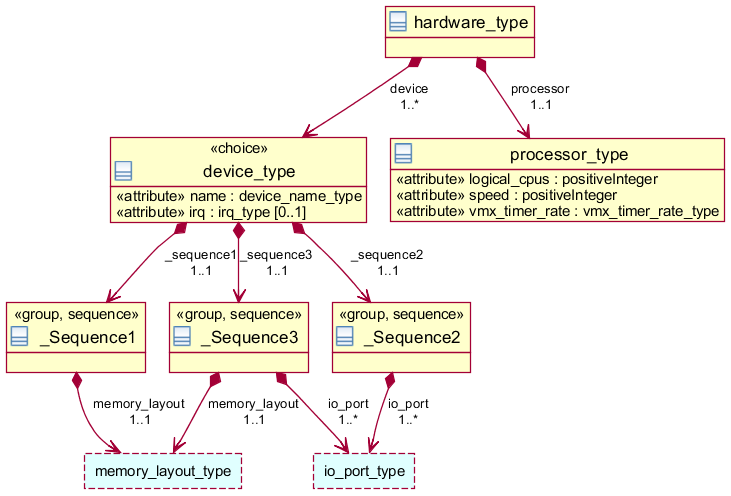
\includegraphics[width=\textwidth]{images/xml_hardware.png}
	\caption{Hardware policy}
\end{figure}
\input{hardware.tex}

\subsection{Kernel}
\begin{figure}[h]
	\centering
	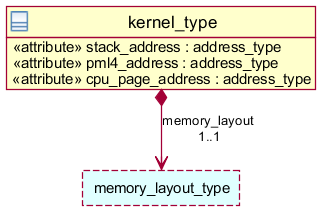
\includegraphics[scale=0.6]{images/xml_kernel.png}
	\caption{Kernel policy}
\end{figure}
\input{kernel.tex}

\subsection{Binaries}
\begin{figure}[h]
	\centering
	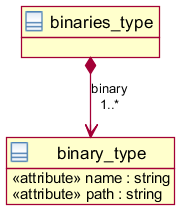
\includegraphics[scale=0.6]{images/xml_binary.png}
	\caption{Binaries policy}
\end{figure}
\input{binary.tex}

\subsection{Subjects}
\begin{sidewaysfigure}[hp]
	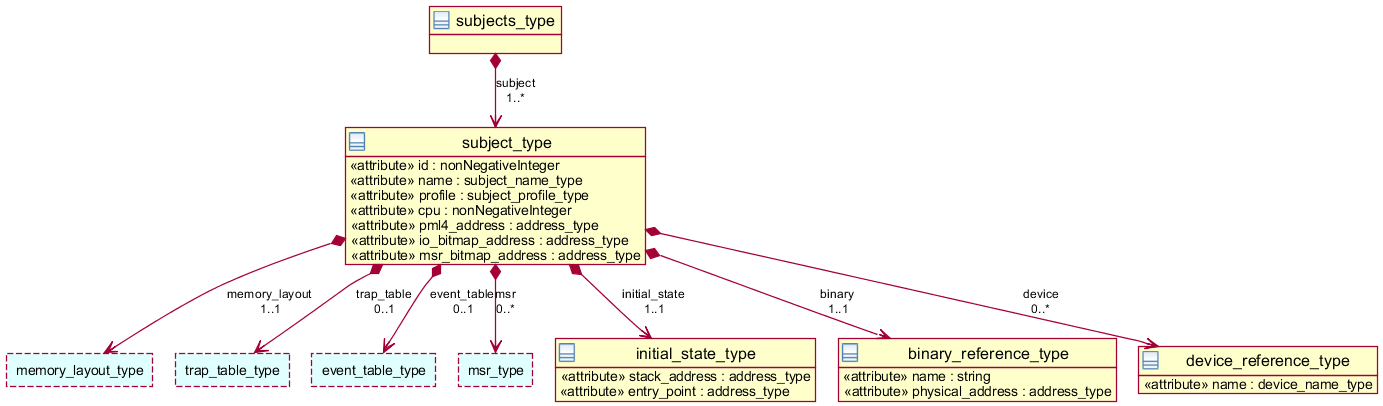
\includegraphics[width=\textwidth]{images/xml_subject.png}
	\caption{Subjects policy}
\end{sidewaysfigure}
\input{subject.tex}

\subsection{Scheduling}
\begin{figure}[h]
	\centering
	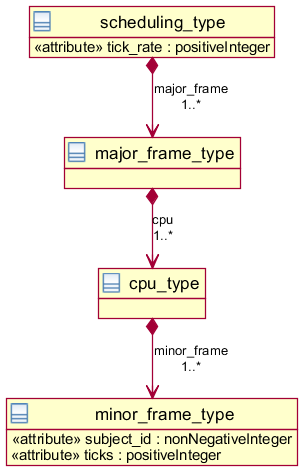
\includegraphics[scale=0.6]{images/xml_scheduling.png}
	\caption{Scheduling policy}
\end{figure}
\input{scheduling.tex}


\section{Subject}\label{sec:impl-subject}
Subjects are the main components that are executed on top of the kernel, as
described in section \ref{sec:design-subject}. They are represented using two
main data structures: subject specification and subject state.

\subsection{Specification}
A subject is specified in the global system policy. The XML specification
precisely defines the execution environment and granted resources. The
information that is relevant to the kernel is part of the compiled policy.
Listing \ref{lst:skp-subjects} presents the SPARK type specification into which
all subject specific policy parts are transformed. The specification of a
subject is static and cannot be changed at runtime.

\lstinputlisting[
	language=ada,
	linerange={14-33},
	label=lst:skp-subjects,
	caption=SPARK subject spec type]
	{../tools/policy/templates/skp-subjects.adb}

\subsection{State}
The system state related to a subject must encompass all resources that it can
control directly or indirectly. This is necessary to enable the scheduler to
preempt a subject by preserving its state and seamlessly resume execution at a
later stage by restoring the previously saved state.

Additionally, separation of subjects demands that unintended information flow
due to subject switching must be prevented. This is only achievable if the
subject state that is saved and restored encompasses every element of the
systems environment that is accessible by more than one subject. While the Intel
VMX extensions save and restore parts of the subject state automatically to and
from the associated VMCS on VMX transition, others must be handled manually by
the kernel. Listings \ref{lst:sk-subject-state} and \ref{lst:sk-cpu-registers}
show the record types used by the Kernel to maintain the state of a subject.

\lstinputlisting[
	language=ada,
	linerange={39-56},
	label=lst:sk-subject-state,
	caption=SPARK subject state type]
	{../common/src/sk.ads}

\lstinputlisting[
	language=ada,
	linerange={18-35},
	label=lst:sk-cpu-registers,
	caption=SPARK CPU registers type]
	{../common/src/sk.ads}

A SM\index{SM} subject may access the state of a given subject. This enables
the SM to alter a subject's state and thus perform emulation. Because a subject
is not allowed to access the VMCS structure of another subject, the kernel also
copies register values managed automatically by VMX\index{VMX} into the
in-memory subject state to enable modification by the SM subject.

During subject setup, the state is first set to a pristine value. This is done
by assigning the \texttt{Null} subject state constants shown by listings
\ref{lst:sk-null-subject-state} and \ref{lst:sk-null-cpu-registers} to all
state variables.

\lstinputlisting[
	language=ada,
	linerange={85-100},
	label=lst:sk-null-subject-state,
	caption=SPARK null subject state constant]
	{../common/src/sk.ads}

\lstinputlisting[
	language=ada,
	linerange={102-118},
	label=lst:sk-null-cpu-registers,
	caption=SPARK null CPU registers constant]
	{../common/src/sk.ads}

The initialization of the subject state is then completed by copying the code
entry point and the address of the stack from the specification.  These values
are declared in the system policy as part of the subject initial state and can
be obtained automatically from a native subject binary by using the
\texttt{skconfig} tool (see section \ref{subsec:subject-binary-analysis}).


\section{Kernel}
\subsection{Init}\label{subsec:init}
After reset of a x86 system, the processor begins executing code at physical
address \texttt{ffff:0000}, which is mapped to the PC
BIOS\index{BIOS}\footnote{Basic Input/Output System}. The BIOS first performs
tests and initialization routines and then searches for a bootable storage
media. If found, the BIOS copies the first sector of the storage media to
physical address \texttt{0000:7C00} and jumps to this address (i.e. starts
executing code at this address). This is where the system bootloader comes to
live which is responsible to boot operating systems according to its
configuration. Many bootloaders first load additional code from the storage
media and then prepare the environment for OS execution.

The Muen seperation kernel is compliant to the multiboot specification, version
0.6.96 \cite{multiboot}. The multiboot standard is used to uniformly boot
different operating system kernels by multiboot-aware bootloaders.
The Muen kernel exports the required multiboot header within the first 8192
bytes of the OS image. The bootloader loads the OS image into memory according
to the information found in the header and jumps to the physical kernel entry
point specified in this header.

It is the bootloader's task to prepare the system state as demanded by the
multiboot standard, see \cite{multiboot} section 3.2 for details. The system
kernel can except the system to be in this state. After the Muen kernel comes to
live, it performs additional steps before jumping into the main SPARK kernel.
This initial startup code is written in Assembly and conducts the following
tasks:
\begin{enumerate}
	\item Copy the AP trampoline to low-memory, see section
		\ref{subsec:mp-support} \item Initialize per-CPU VMXON regions
	\item Initialize subject VMCS regions
	\item Enable PAE\index{PAE}\footnote{Physical Address Extension}
	\item Initialize per-CPU kernel pagetables
	\item Enable IA-32e mode and execute-disable (NX)
	\item Enable paging, write protection, caching and native FPU error
		reporting
	\item Set up 64-bit GDT\index{GDT}\footnote{Global Descriptor Table}
	\item Set up Page-Attribute Table (PAT)
	\item Set up kernel stack
	\item Initialize Ada runtime
	\item Jump into kernel main
\end{enumerate}
After this initial steps are executed, the system is in 64-bit IA-32e mode and
all prerequisites are met to enable VMX root operation.

\subsection{Scheduling}
\begin{figure}[h]
	\centering
	\begin{tikzpicture}[minimum height=0.6cm]
	\node (sch) [bluebox]                {Scheduler};
	\node (knl) [bluebox, left=of sch]   {Kernel Main};
	\node (pln) [apribox, above=of sch]  {Scheduling Plan};
	\node (sub) [greenbox, right=of sch] {Subject};
	\node[gray!80, font=\scriptsize] at (0.8,2.3) {VMX root};
	\node[gray!80, font=\scriptsize] at (2.6,2.3) {VMX non-root};

	\draw[arrow] (knl) to (sch);
	\draw[arrow] (pln) to (sch);
	\draw[arrow] (sch) to[bend right=65] node[auto] {VM enter} (sub);
	\draw[arrow] (sub) to[bend right=65] node[auto] {VM exit}  (sch);
	\draw[thin, dotted, gray] (1.6,-1.5) to (1.6,2.5);
\end{tikzpicture}

	\caption{Kernel scheduler}
	\label{fig:kernel-scheduler}
\end{figure}

\subsection{Traps}
\subsection{Exceptions and Interrupts}
\begin{figure}[h]
	\centering
	\begin{tikzpicture}
	\node[graybox] (han) {\textbf{3} Handle IRQ};
	\node[above=2mm of han] (mue) {Muen SK};

	\begin{pgfonlayer}{background}
		\node[bluebox, minimum width=3cm, minimum height=1.7cm] (mub) [fit = (han) (mue)] {};
	\end{pgfonlayer}

	\node[greenbox, minimum width=3cm, minimum height=1.7cm, above=of mub] (sub) {Subject};
	\node[apribox, left=15mm of mub] (irq) {Keyboard};

	\draw[arrow] (irq) to node[auto] {\textbf{1} IRQ 1} (mub);
	\draw[arrow] (sub.225) to node[auto, swap] {\textbf{2} VM exit} (mub.135);
	\draw[arrow] (mub.45) to node[auto, swap] {\textbf{4} Inject event} (sub.315);
\end{tikzpicture}

	\caption{External interrupt handling}
	\label{fig:external-interrupt}
\end{figure}

\subsection{Multicore support}\label{subsec:mp-support}
The Muen separation kernel makes use of all logical processors available in a
system. The processor count of a specific hardware platform is specified in the
system policy, see section \ref{subsec:hardware}. This section describes how the
multicore setup is done on kernel startup.

Modern PC systems comply to the Intel MultiProcessor (MP\index{MP})
specification. In short, the Intel MP specification is an open-standard
describing enhancements to both operating systems and firmware to be able to
init, boot and operate x86 multiprocessor systems. For more information see
\cite{intel:mp}.

After the hardware completed its part of the MP specification, one processor
has been negotiated to be the bootstrap processor (BSP\index{BSP}). All other
logical processors, called application processors (AP\index{AP}), halt until
they receive a specific inter-processor interrupt (IPI\index{IPI}) sequence.

\begin{figure}[h]
	\centering
	\begin{tikzpicture}
	\node[greenbox, minimum width=9cm] (mem) {System Memory};

	% SK 0
	\node[graybox, minimum width=2.8cm, below=1cm of mem.south west, anchor=north west] (pc1) {Per-CPU storage};
	\node[graybox, minimum width=2.8cm, below=1mm of pc1] (st1) {Stack};
	\node[above=2mm of pc1] (mu1) {Muen SK};
	\begin{pgfonlayer}{background}
		\node[bluebox, minimum width=3cm, minimum height=1.7cm] (mb1) [fit = (pc1) (st1) (mu1)] {};
	\end{pgfonlayer}

	\node[apribox, minimum width=3cm, below=5mm of mb1, label=below:\emph{BSP}] (cp1) {CPU0};

	\draw[arrow, gray] (mb1) to node[auto, gray] {LAPIC} (cp1);

	% SK 1
	\node[graybox, minimum width=2.8cm, below=1cm of mem.south east, anchor=north east] (pc2) {Per-CPU storage};
	\node[graybox, minimum width=2.8cm, below=1mm of pc2] (st2) {Stack};
	\node[above=2mm of pc2] (mu2) {Muen SK};
	\begin{pgfonlayer}{background}
		\node[bluebox, minimum width=3cm, minimum height=1.7cm] (mb2) [fit = (pc2) (st2) (mu2)] {};
	\end{pgfonlayer}

	\node[apribox, minimum width=3cm, below=5mm of mb2, label=below:\emph{AP}] (cp2) {CPU1};

	\draw[arrow, gray] (cp2) to node[auto, gray] {LAPIC} (mb2);

	% Inter-core
	\draw[arrow, gray] (mb1) to node[gray, auto] {INIT-SIPI-SIPI} (mb2);
\end{tikzpicture}

	\caption{Multicore architecture}
	\label{fig:mp-overview}
\end{figure}

The BSP starts executing code as describe in section \ref{subsec:init}. The
init code initializes the system and jumps into the main SPARK kernel. The
kernel running on the BSP is responsible to bootstrap the other application
processors. It first enables its local APIC\index{APIC} to be able to send
inter-processor interrupts to the halted AP processors. To wakeup the APs, the
INIT-SIPI-SIPI IPI sequence must be sent to their APICs, as described in the MP
specification. See also figure \ref{fig:mp-overview} for an illustration of
this process. The SIPI IPI contains the physical address vector of the
trampoline code copied to low-memory by the init code. The AP processors jump
to this code after wakeup. The trampoline performs the following steps:

\begin{enumerate}
	\item Set up 32-bit GDT\index{GDT}
	\item Switch CPU to protected mode
	\item Initialize DS and SS segments
	\item Jump to the AP entry point in the init code
\end{enumerate}

These steps initialize the APs to the same architectural state as the
bootloader did for the BSP: 32-bit protected mode with paging disabled.
Therefore, the final step is to let the AP processors jump to the identical
init code described in section \ref{subsec:init}.

\subsubsection{Per-kernel memory}
The Muen kernels operate fully symmetrical, i.e. code running on the different
logical processors is (binary) identical. Nevertheless, each kernel owns a
distinct stack page and also a page to store per-CPU data. This however is fully
transparent to the kernels as their virtual stack and global storage addresse
values are the same. This is achieved by using different page table structures
for each kernel. Page tables are created by the policy tool and setup on system
startup by the init code. The main kernel has no access to these structures in
memory and does not bother with memory management.

\subsubsection{Synchronization} Since synchronization is error-prone and it is
desirable to reduce inter-core dependencies as much as possible, the Muen
kernel tries to avoid locks and other synchronization primitives. Nevertheless
minimal synchronization is required at certain key points in the code. This
section describes the spinlock and barrier mechanisms used by the kernel.

\paragraph{Spinlock}
The spinlock implementation uses the \texttt{XCHG} processor instruction to
atomically swap the value one with the contents of a lock variable in memory.
If the result of the set operation is zero, no other core currently holds the
lock and it is successfully acquired. If the result is one, the lock is
currently busy and the core must spin and retry again.

Inside the lock's busy loop the \texttt{PAUSE} instruction is used to improve
performance and resource utilization on CPUs with hyper-threading
(HTT\index{HTT}) enabled TODO:REF.

\paragraph{Barrier}
As described in section \ref{subsec:scheduling}, to guarantee temporal
separation, the scheduling plans on the different logical processors must be
synchronized on major frame transition.

This is achieved by ...

\subsection{Events}
\begin{figure}[h]
	\centering
	\begin{tikzpicture}
	% SK 0
	\node[graybox] (ha1) {Handle Hypercall};
	\node[above=2mm of ha1] (mu1) {Muen SK};
	\begin{pgfonlayer}{background}
		\node[bluebox, minimum width=3cm, minimum height=1.7cm] (mb1) [fit = (ha1) (mu1)] {};
	\end{pgfonlayer}

	\node[apribox, minimum width=3cm, below=5mm of mb1] (cp1) {CPU0};
	\node[greenbox, minimum width=3cm, minimum height=1.7cm, above=of mb1] (su1) {Subject};

	\draw[arrow] (su1.225) to node[auto, swap] {\textbf{1}} (mb1.135);
	\draw[arrow] (mb1.45) to node[auto, swap] {\textbf{4}} (su1.315);
	\draw[<->, thick] (cp1) to node[auto] {LAPIC} (mb1);

	% SK 1
	\node[graybox, right=2.6cm of ha1] (ha2) {Handle Hypercall};
	\node[above=2mm of ha2] (mu2) {Muen SK};
	\begin{pgfonlayer}{background}
		\node[bluebox, minimum width=3cm, minimum height=1.7cm] (mb2) [fit = (ha2) (mu2)] {};
	\end{pgfonlayer}

	\node[apribox, minimum width=3cm, below=5mm of mb2] (cp2) {CPU1};
	\node[greenbox, minimum width=3cm, minimum height=1.7cm, above=of mb2] (su2) {Subject};

	\draw[arrow] (mb2.135) to node[auto, swap] {\textbf{2}} (su2.225);
	\draw[arrow] (su2.315) to node[auto, swap] {\textbf{3}} (mb2.45);
	\draw[<->, thick] (cp2) to node[auto] {LAPIC} (mb2);

	% Inter-core
	\draw[<->, thick] (mb1) to node[auto] {IPI} (mb2);
	\draw[vecarrow] (su1.15) to node[auto] {Request page} (su2.165);
	\draw[vecarrow] (su2.195) to node[auto] {Response page} (su1.345);
\end{tikzpicture}

	\caption{Inter-core events}
	\label{fig:inter-core-events}
\end{figure}

\section{Build}
TODO: explain the complete process, target dependencies and implemented tools.
\begin{figure}[h]
	\centering
	\begin{tikzpicture}[minimum height=0.6cm]
	\node (src) [apribox]               {Source Format};
	\node (mrg) [bluebox, right=of src] {Merger};
	\node (exp) [bluebox, right=of mrg] {Expander};
	\node (fma) [apribox, right=of exp] {Format A};
	\node (alo) [bluebox, right=of fma] {Allocator};
	\node (fmb) [apribox, below=of alo] {Format B};
	\node (val) [bluebox, left=of fmb]  {Validator};
	\node (sge) [bluebox, left=of val]  {Structure Generators};

	\node (spk) [graybox, below=of sge] {Source Specs};
	\node (iob) [graybox, right=of spk] {I/O Bitmaps};
	\node (msc) [graybox, right=of iob, minimum width=1.5cm] {...};
	\node (pta) [graybox, left=of spk] {Page Tables};
	\node (zpa) [graybox, left=of pta] {Zero Page};

	\node (bin) [apribox, below=of spk] {Binaries};

	\node (has) [bluebox, below=of bin] {Hasher};

	\node (sin) [bluebox, below=of has] {Sinfo};

	\node (pak) [bluebox, below=of sin] {Packer};

	\node (img) [apribox, below=of pak] {System Image};

	\draw[arrow] (src) -- (mrg);
	\draw[arrow] (mrg) -- (exp);
	\draw[arrow] (exp) -- (fma);
	\draw[arrow] (fma) -- (alo);
	\draw[arrow] (alo) -- (fmb);
	\draw[arrow] (fmb) -- (val);
	\draw[arrow] (val) -- (sge);

	\draw[arrow] (sge) -- (spk);
	\draw[arrow] (sge) -- (iob);
	\draw[arrow] (sge) -- (msc);
	\draw[arrow] (sge) -- (pta);
	\draw[arrow] (sge) -- (zpa);

	\draw[arrow] (spk) -- (bin);

	\draw[arrow] (bin) -- (has);
	\draw[arrow] (has) -- (sin);
	\draw[arrow] (sin) -- (pak);

	\draw[arrow] (msc) -- (pak);
	\draw[arrow] (iob) -- (pak);
	\draw[arrow] (iob) -- (pak);
	\draw[arrow] (pta) -- (pak);
	\draw[arrow] (zpa) -- (pak);

	\draw[arrow] (pak) -- (img);
\end{tikzpicture}

	\caption{Build process}
	\label{fig:build-process}
\end{figure}

\subsection{Policy compilation}
The \texttt{skpolicy} tool compiles the XML system policy outlined in section
\ref{sec:policy} to different output formats as shown in figure
\ref{fig:policy-compilation}.

\begin{figure}[h]
	\centering
	\begin{tikzpicture}
	\node (pol) [greenbox]                            {Policy};
	\node (skp) [apribox, below=of pol]               {skpolicy};
	\node (sou) [bluebox, below=of skp, xshift=1.5cm] {Source specs};
	\node (pag) [bluebox, left=of sou]                {Page tables};
	\node (iob) [bluebox, left=of pag]                {I/O bitmaps};
	\node (msr) [bluebox, right=of sou]               {MSR bitmaps};

	\draw[arrow] (pol) to (skp);
	\draw[arrow] (skp) to (sou);
	\draw[arrow] (skp) to (msr);
	\draw[arrow] (skp) to (pag);
	\draw[arrow] (skp) to (iob);
\end{tikzpicture}

	\caption{Policy compilation}
	\label{fig:policy-compilation}
\end{figure}

The generated subject page tables, I/O and MSR bitmaps are included in the final
system image by the \texttt{skpacker} utility explained in the following section
\ref{subsec:image-packaging}. These files are all in binary form and correspond
to the format mandated by the respective Intel SDM chapters (TODO:REF). Page
tables are generated for subjects as well as for the kernel itself.

The generated SPARK and Assembly source specifications are included in the
kernel directly. These specifications provide the kernel with the following
information:

\begin{itemize}
	\item \emph{IRQ routing specification}\\
		Used by the kernel to program the system's I/O APIC for interrupt
		routing.
	\item \emph{Kernel address constants}\\
		Define kernel stack, page table and per-CPU storage memory addresses.
	\item \emph{Scheduling plans for all CPU cores}\\
		The scheduling plans are indexed by the logical processor's APIC ID.
		Each kernel copies its associated scheduling plan to the per-CPU storage
		area on initialization.
	\item \emph{Subjects specification}\\
		Defines all subjects and their parameters, see policy section
		\ref{subsec:subjects}.
	\item \emph{Packer specification}\\
		Defines the configuration used for the \texttt{skpacker} tool outlined
		in the following section \ref{subsec:image-packaging}.
\end{itemize}

\subsection{Subject binary analysis}\label{subsec:subject-binary-analysis}
The \texttt{skconfig} tool uses the Binary File Descriptor (BFD\index{BFG})
library to analyze subject binaries and creates appropriate XML\index{XML}
policy specifications from it, see figure \ref{fig:object-analysis}. This is
useful to generate the initial state and the memory layout directly from a
native subject binary instead of writing it by hand. The tool extracts stack
address, entry point and memory layout from a subject binary.

\begin{figure}[h]
	\centering
	\begin{tikzpicture}
	\node (obj) [bluebox]                {Binary object};
	\node (skc) [apribox,  below=of obj] {skconfig};
	\node (xml) [greenbox, below=of skc] {XML specification};

	\draw[arrow] (obj) to (skc);
	\draw[arrow] (skc) to (xml);
\end{tikzpicture}

	\caption{From binary object to XML specification}
	\label{fig:object-analysis}
\end{figure}

The exctracted subject initial state and memory layout XML specifications can be
included in the system policy before compilation by the \texttt{skpolicy} tool.
The generated memory layout is only as permissive as required by the original
subject binary. For example, the memory region mapped for executable code
(the \texttt{.text} section) will be executable but non-writeable. This is in
contrast to just providing a big enough memory region with all permissions to
the subject with no exact mapping of binary sections to memory access
permissions (i.e. read, write, execute).

\subsection{Image packaging}\label{subsec:image-packaging}
The \texttt{skpacker} tool is responsible to assemble the final bootable system
image from the parts produced in the previous build steps. Figure
\ref{fig:image-packaging} illustrates the process. The tool includes the special
packer source specification created from the system policy. This specification
includes information about subject binaries and their physical address in the
final image.

\begin{figure}[h]
	\centering
	\begin{tikzpicture}
	\node (knl) [bluebox]                              {Kernel binary};
	\node (sub) [bluebox, left=of knl]                 {Subject binaries};
	\node (pag) [bluebox, left=of sub]                 {Page tables};
	\node (bit) [bluebox, right=of knl]                {Bitmaps};
	\node (skp) [apribox, below=of knl, xshift=-1.5cm] {skpacker};
	\node (spe) [bluebox, left=of skp]                 {Packer spec};
	\node (sys) [greenbox, below=of skp]               {System image};

	\draw[arrow] (pag) to (skp);
	\draw[arrow] (sub) to (skp);
	\draw[arrow] (knl) to (skp);
	\draw[arrow] (bit) to (skp);
	\draw[arrow] (skp) to (sys);
	\draw[arrow] (spe) to (skp);
\end{tikzpicture}

	\caption{System image packaging}
	\label{fig:image-packaging}
\end{figure}

The remaining configuration is extracted from the source specification provided
to the kernel. Listing \ref{lst:skpacker} shows the output of a
\texttt{skpacker} run with the example system described in section
\ref{sec:example-system}. The fist column in the output designate physical
addresses in memory. The second column specifies the type of the packaged file
at this specific memory location. The abbreviations have the following meaning:

\begin{itemize}
	\item \emph{PML4} The file at this address designates a page table
		structure. It is either a page table for a kernel or for a subject. The
		kernels running on the different logical processors have different page
		tables to allow distinct stack and per-CPU storage pages transparently.
	\item \emph{IOBM} The file is a subject I/O bitmap. Specifies which I/O
		ports a subject is allowed to access.
	\item \emph{MSBM} The file is a subject MSR bitmap. Specifies which MSRs a
		subject is allowed to access.
	\item \emph{BIN} The file is a subject (raw) binary.
\end{itemize}

\begin{lstlisting}[
	caption=Example output of skpacker tool,
	label=lst:skpacker,
	frame=none,
	numbers=none]
         Packaging kernel image 'obj/kernel'
         0000000000200000 [PML4] kernel (0)
         0000000000204000 [PML4] kernel (1)
         0000000000208000 [PML4] kernel (2)
         000000000020c000 [PML4] kernel (3)
         0000000000210000 [PML4] tau0
         0000000000214000 [IOBM] tau0
         0000000000216000 [MSBM] tau0
         0000000000217000 [BIN ] tau0
         0000000000240000 [PML4] vt
         0000000000244000 [IOBM] vt
         0000000000246000 [MSBM] vt
         0000000000247000 [BIN ] vt
         0000000000270000 [PML4] crypter
         0000000000274000 [IOBM] crypter
         0000000000276000 [MSBM] crypter
         0000000000277000 [BIN ] crypter
         00000000002a0000 [PML4] sm
         00000000002a4000 [IOBM] sm
         00000000002a6000 [MSBM] sm
         00000000002a7000 [BIN ] sm
         00000000002d0000 [PML4] xv6 (EPT)
         00000000002d4000 [IOBM] xv6
         00000000002d6000 [MSBM] xv6
         00000000002d7000 [BIN ] xv6
\end{lstlisting}

\section{Example system}\label{sec:example-system}
\begin{figure}[h]
	\centering
	\begin{tikzpicture}[node distance=0.33cm]
	\node[redbox, text width=1.5cm, minimum width=2cm, minimum height=2cm] (vts) {VT Native};
	\node[redbox, text width=1.5cm, minimum width=2cm, minimum height=2cm, left=of vts] (cry) {Crypter Native};
	\node[redbox, text width=1.5cm, minimum width=2cm, minimum height=2cm, left=of cry] (smn) {Subject Monitor Native};
	\node[blackbox, text width=1.5cm, minimum width=2cm, minimum height=2cm, left=of smn] (xv6) {xv6 VM};
	\node[bluebox, minimum height=1cm, minimum width=9cm, text width=6cm] at (-3.5,-2.5) (mue) {Muen Separation Kernel};

	\draw[gray] (-8,-2.25) to (1,-2.25);
	\draw[gray] (-5.84,-2.25) to (-5.84,0);
	\draw[gray] (-3.50,-2.25) to (-3.50,0);
	\draw[gray] (-1.14,-2.25) to (-1.14,0);
\end{tikzpicture}

	\caption{Example system}
	\label{fig:example-system}
\end{figure}

\chapter{Conclusion}
This chapter provides a summary of the contributions and an outlook on possible
future work.

\section{Contributions}
The main results of this work are the separation kernel design and prototype as
well as the accompanying proof artifacts. To our knowledge it is the first
publicly and freely available separation kernel for the Intel
x86/IA-32e\index{IA-32e} architecture.

Use of the SPARK language and tools for the realization of the Muen kernel
provides the base for a high assurance implementation. Full absence of
runtime errors and some additional properties have been proven. Since the SPARK
tools are freely available, anyone can reproduce the proofs in their own
environment.

Focus on use of the latest Intel hardware virtualization features and emphasis
on a simple design have resulted in a small code size. The kernel is thus well
suited for review. It is a sound basis for further formal verification such as
the application of the theorem prover Isabelle/HOL via the HOL-SPARK
verification environment \cite{berghofer:OASIcs:2012:3587}.

An example system modeled after a realistic component-based use-case has been
implemented to demonstrate the viability of the design and the usability of the
kernel prototype. Multicore support makes better use of modern processors that
feature an increasing number of logical CPUs.

The complete source code, build environment, supporting tools and documentation
are provided, allowing independent review of the complete TCB.

\section{Future work}
The following list gives a somewhat ordered overview of possible future
enhancements to the Muen separation kernel:

\begin{itemize}
	\item Covert/Side-Channel analysis
	\item Cache coloring
	\item Linux virtualization
	\item Hardware passthrough/PCIe virtualization
	\item Dynamic resource management
	\item Multicore subjects
	\item Performance optimization
	\item Power Management
	\item Formal verification
	\item Fully virtualized subjects/Windows virtualization
\end{itemize}

The following sections describe some of the more interesting items.

\subsection{Covert/Side-channel analysis}
Since the main purpose of a separation kernel is the isolation of subjects, any
unintended channel that enables information flow must be prohibited or at least
reduced to an acceptable data rate.

The first step in preventing such flows is to identify potential covert and
side-channels in the kernel. This includes a systematic and thorough analysis of
the underlying hardware platform. Special care must be taken to evaluate the
interaction of the kernel with the hardware since minor differences in
interpretation of the specification can lead to unintended side-effects. A very
deep knowledge and understanding of the Intel x86 architecture is required for
such an analysis.
TODO:Ref

\subsubsection{Cache coloring}
A well-known source of high-bandwith side-channels are processor caches. One
method to prevent this channel is called \emph{cache coloring}. The main concept
is to partition the cache into disjoint groups and assigning a color to each of
the groups. TODO:Cache coloring ref

In a second step each subject is associated with a color. All subjects of a
given color share the same cache partition. In turn subjects of differing color
have no access to the same cache locations, which means the cache cannot be used
as a side-channel.

This mechanism could be implemented by extending the policy compilation tool
without changes to the kernel.

\subsection{Linux subject}
Porting the Linux kernel to run as a subject on the Muen separation kernel would
enable the execution of a large number of Linux user-space applications. This
would drastically increase the number of real world use-cases, that a system
using the Muen kernel could be applied to.

Leveraging the VM profile, which allows a subject to perform memory management
via EPT (see section \ref{subsubsec:ept}), reduces the porting effort. Changes
to the Linux boot process are needed, since it is quite involved. The Linux
kernel implements an architecture-dependent boot protocol that is documented in
TODO:Ref.

Combined with the \emph{hardware passthrough} enhancement, Linux could be used
to control virtually any PCI(e) device. This would add the abundant hardware
support of the Linux kernel to systems based on the separation kernel, with a
comparably small increase in kernel complexity.

\subsection{Hardware pass-through/PCIe virtualization}
Even though the separation kernel has support for resources, that can be
accessed using port and memory-mapped I/O, newer hardware devices are attached
to a PCI bus. Prior to their usage, such devices must be configured using a
mechanism called the PCI configuration space. Since this ressource allows to
(re-)configure PCI devices, the kernel must be in charge of device management
like initial setup.

Subjects performing device enumeration to discover the PCI topology would need
a virtualized view of the PCI bus or be altered to not perform disallowed access
to the PCI configuration space.

Additional measures need to be implemented to enable subject assignment and safe
usage of PCI devices. Most PCI devices support Direct Memory Access (DMA), which
allows them to directly access all data in physical memory. Secondly, a PCI
device is not restricted to a specific hardware interrupt but can be instructed
to trigger any interrupt. Intel's VT-d technology, as briefly mentioned in
section \ref{subsubsec:vtd}, provides mechanisms to implement the necessary
isolation functions.

Implementing these enhancements using VT-d should keep the kernel complexity at
an acceptable level.

\subsection{Dynamic resource management}
Currently, resource management is static and there is little flexibility. All
system parameters must be explicitly declared in the policy. Switching between
pre-defined scheduling plans is the only property changeable at runtime. While
this allows to tightly control and validate a system via the policy, all
assigned resources are indispensable even though some of them may not be in use
during a particular period.

For example, a system consisting of multiple different VM subjects with their
respective operating systems need multiple gigabytes of memory when running.
In a static system configuration, all the assigned memory is committed and
reserved even though only one of the VMs might be in active use. A system that
would allow dynamic launching and stopping of subjects, only the resources of
the effectively running subjects would be in use.

This can be achieved by extending the trusted subject $\tau$0. It has the same
trust-level as the kernel and forms part of the TCB. Via an appropriate
interface it can update parts of the policy and instruct the kernel to perform
the necessary actions to enforce the changes.

\subsection{Formal verification}
By implementing the kernel in SPARK and proving the absence of runtime errors,
we have shown that the kernel is free from exceptions. While these proofs
provide some evidence to the correctness claim of the implementation, the
application of these particular formal methods do not provide any assurances
beyond the error free execution of the kernel. Proving functional properties
such as the correspondence of the scheduler to a given formal specification is
necessary to further raise the confidence in systems based on the Muen kernel.

A link between the SPARK tool suite and the interactive proof assistant
Isabelle/HOL exists in the form of the \emph{HOL-SPARK} verification
environment \cite{berghofer:OASIcs:2012:3587}. Isabelle would allow to prove
the formal correctness of the Muen separation kernel. The viability of this
approach has been demonstrated by the seL4 project \cite{Klein_EHACDEEKNSTW_09}.



\printindex{}

\bibliographystyle{plain}
\bibliography{report}

\end{document}
